% Subsection intro. Elaborate on origins of DP. Why it is useful.
Data scientists strive to understand the general properties of a population. 
To answer questions concerning the etiology of a disease, factors contributing to a societal phenomenon, or the consequences of an economic policy, researchers collect data from individual people. They then process this data to calculate population-level statistics and propose solutions based on these aggregated statistics.
Ensuring the privacy of individuals who have contributed to these studies is of utmost importance from both ethical and legal perspectives.
In fact, the intended goal of all scientific studies is to collect valuable information about the targeted population not individuals within the population. 
However, it is impossible to learn useful information about a population while learning \textit{nothing} about individuals, leading to a paradox between usefulness of a dataset (\ie utility) and its privacy. 
Differential Privacy (DP) addresses this paradox by quantifying the extent of privacy leakage for individuals in a dataset when publishing its statistics.
Within the framework of Differential Privacy (DP), the aforementioned paradox transforms into an adjustable trade-off between the utility of data and the preservation of privacy. 

In the rest of this section, we provide the formal definition of differential privacy, highlight its main properties, and explore its potential application in the domain of traffic shaping.


%
%% 
%% Definition
%%
%


\subsection{Definitions}\label{subsec:background-dp-definitions}
A database $D$ has a fixed number of entries, where each individual data point is stored in one entry.
Following the notation proposed by Dwork \etal \cite{dwork2014algorithmic}, we represent databases by their histograms: $D \in \dbSpace$. 
In this representation, every entry $D_i$ of the database $D$ represents the number elements of type $i \in \mathcal{X}$.
\\  
Within the DP context, \textit{query} is defined as a function that operates on a database. 
Any computation performed on a database, regardless of its codomain, can be regarded as a query executed on that database.
The primary objective of differential privacy is to offer meaningful population-level information for queries executed on a database, while protecting the privacy of individual data points in the database.
Intuitively, small changes in a database should not significantly impact the outcome of a query.
To further clarify the terms "small changes" and "significant impact", we provide definitions for neighboring databases and query function sensitivity, respectively.
We measure the difference between two databases with a distance metric $\rho(D, D')$.
\begin{definition}[Neighboring databases]
  Given a distance metric $\rho$, DP refers to two databases $D, D' \in \dbSpace$ as neighboring databases, if and only if $\rho(D, D') \leq 1$.             
\end{definition}
\noindent In the standard DP definition, the distance metric is simply the number of different data entries in two databases (\ie Hamming distance).
However, Chatzikokolakis \etal \cite{chatzikokolakis2013broadening} show that DP applies to a general definition of distance metrics.
To quantify the extent to which a single data point can influence the outcome of a query in the worst-case, DP introduces the concept of sensitivity. 
\begin{definition}[$l_p$-Sensitivity]
  \label{def:norm-sensitivity}
  The $l_p$-sensitivity of a query function $f$ is:
  \begin{equation*}
    \Delta_p f = \max_{D, D'} \|f(D) - f(D')\|_p 
  \end{equation*}
where $\rho(D, D') \leq 1$ (\ie $D$ and $D'$ are neighboring databases).
\end{definition}
\noindent
Differential Privacy involves randomization of query outputs. DP defines a randomized algorithm as follows.
\begin{definition}[Randomized algorithm]
  \label{def:randomized-algorithm}
  A randomized algorithm $M$ with the domain $A$ and discrete range $B$, for any given $a \in A$ and $b \in B$ outputs $M(a)= b$ with probability of $(M(a))_b$.
\end{definition}

With all the necessary components in place, we are now prepared to present the formal definition of differential privacy.
\begin{definition}[Differential privacy]
  \label{def:dp}
  A randomized algorithm $M: \dbSpace \rightarrow \mathbb{R}$ is $(\varepsilon, \delta)$-differentially private if for all ${S} \subseteq Range(M)$ and for  all $D, D' \in \dbSpace$ such that $\rho(D, D') \leq 1$, we have:
  \begin{equation*}
    \Pr[M(D) \in S] \leq \exp(\varepsilon)\Pr[M(D') \in S] + \delta
  \end{equation*}
\end{definition}
\noindent
Indeed, Differential Privacy (DP) is a definition rather than a specific algorithm.
It provides a framework for ensuring privacy guarantees in various randomized algorithms. Multiple randomized algorithms can achieve $(\varepsilon, \delta)$-privacy for a given set of databases, each with different characteristics. 
Intuitively, given an output, with probability $1-\delta$, the log likelihood ratio of running the algorithm $M$ on databases $D$ and $D'$ is bounded by $\varepsilon$.
This bound ensures that the presence or absence of any individual's data in the database has a limited impact on the likelihood of obtaining a particular output.
The smaller $\varepsilon$ implies that both neighboring databases are equally likely to generate the output, resulting in more privacy.
The parameter $\varepsilon$ is commonly referred to as \textit{privacy loss} within the context of DP.
The parameter $\delta$ determines the failure probability of a differential private mechanism and is typically expected to have a small value (\ie smaller than $10^{-5}$).


%
%% 
%% Properties
%%
%

\subsection{Properties}\label{subsec:background-dp-properties}
We, now, explore the key properties of Differential Privacy as a privacy framework.


% ROBUSTNESS TO AUXILIARY INFORMATION.
\subsubsection{Robustness to auxiliary information}
\label{subsubsec:dp-auxiliary}
The definition of Differential Privacy does not make any assumptions regarding the prior knowledge of the adversary. 
In other words, regardless of the adversary's prior knowledge, the information gained by the adversary after observing the output of a differentially private algorithm $M$ remains within the bounds specified by Differential Privacy~\cite{dwork2014algorithmic}. 
\begin{proposition}
  \label{prop:auxiliary}
  Assume that the adversary has a prior $\Pr(D)$ over the set of all possible databases $D, D' \in \dbSpace$. Given the output $S$ of a $(\varepsilon, \delta)$-DP algorithm $M: \dbSpace \rightarrow \mathbb{R}$, for all $D, D' \in \dbSpace$ such that $\rho(D, D') \leq 1$, we have: 
  \begin{equation*}
    \frac{\Pr(D|S)}{\Pr(D'|S)} \leq \exp(\varepsilon) \frac{\Pr(D)}{\Pr(D')}
  \end{equation*}
\end{proposition}
In broad terms, robustness to auxiliary information in the context of Differential Privacy is similar to the security semantics of cryptographic algorithms. 
For instance, consider a scenario where an adversary possesses the knowledge that the content of an encrypted message is either a picture of a car or a picture of a tree.
In this case, observing the encrypted message does not provide any additional evidence to indicate which of the two possibilities is more likely to be the true message.
In DP, nevertheless, observing the results of private queries does change the prior knowledge of the adversary.
However, this change remains within the boundaries defined by DP and does not exceed them.

% POST-PROCESSING
\subsubsection{Post-processing}
\label{subsubsec:background-dp-postprocessing}
Differential Privacy guarantees are resilient to post-processing of the output from a DP algorithm.
In fact, in the absence of any additional knowledge, the adversary is unable to undermine the guarantees of Differential Privacy simply by processing the output of the algorithm.
\begin{proposition}
  \label{prop:post-processing}
  Consider $M: \dbSpace \rightarrow R$ as a $(\varepsilon, \delta)$-differentially private algorithm, and let $g: \mathbb{R} \rightarrow \mathbb{R}$ be an arbitrary randomized mapping, then $g(M(.)): \dbSpace \rightarrow \mathbb{R}$ is $(\varepsilon, \delta)$-differentially private. 
\end{proposition}
\noindent
This implies that regardless of the complexity of a procedure, as long as the inputs are differentially private, the output is guaranteed to maintain the same level privacy.
The post-processing property of Differential Privacy can be especially advantageous when dealing with systems that have information bottlenecks, such as situations where results from multiple calculations are aggregated at a single stage.
In such systems, by applying a differentially private algorithm to the information bottleneck, the guarantee of Differential Privacy extends to the output of the entire system. 
We specifically utilize the post-processing property of Differential Privacy in the design of both the {\sys} shaping mechanism and the {\sys} middlebox. 

% PRESERVATION UNDER ADAPTIVE SEQUENTIAL COMPOSITION.
\subsubsection{Self-Composition}\label{subsubsec:background-dp-composition}
The simultaneous release of results from multiple differentially private algorithms maintains the differential privacy guarantee.
This property facilitates the modular construction of differentially private algorithms, allowing multiple DP algorithms to be combined to create more sophisticated and advanced algorithms.
Furthermore, the composition theorem enables us to compute the privacy parameters associated with the sequential release of a differentially private algorithm output, thereby facilitating multiple releases of the same DP output.
There are multiple variants of the composition theorem, and we start with the simplest form of composition.
\begin{proposition}[Basic composition theorem]
\label{prop:basic-composition}
  Let $M_i: \dbSpace \rightarrow \mathbb{R}$ be an $(\varepsilon_i, \delta)$-differentially private algorithm for $i \in [k]$. Then, the combination of these $k$ algorithms, $M_{[k]}: \dbSpace \rightarrow \Pi_{i=1}^{k}\mathbb{R}$ is $(\sum_{i=1}^{k}\varepsilon_i, \sum_{i=1}^{k}\delta_i)$-differentially private.  
\end{proposition}
The basic composition theorem~\cite{dwork2014algorithmic} states that the privacy loss resulting from the combination of multiple differentially private algorithms is equal to the aggregate of their individual privacy losses.
While functional, the basic composition theorem tends to overestimate the privacy loss of combined DP algorithms (see \Cref{prop:rdp-composition}).
The advanced composition theorem offers a more precise and rigorous bound for the aggregated privacy loss incurred by multiple differentially private algorithms. 
\begin{proposition}[Advanced composition theorem]
\label{prop:advanced-composition}
  Let $M_i: \dbSpace \rightarrow \mathbb{R}$ be an $(\varepsilon, \delta)$-differentially private algorithm for $i \in [k]$. Then, the combination of these $k$ algorithms, $M_{[k]}: \dbSpace \rightarrow \Pi_{i=1}^{k}\mathbb{R}$ is $(\varepsilon', k\delta+\delta')$-differentially such that:
  \begin{equation*}
    \forall \delta' \geq 0: \varepsilon' = \sqrt{2k\ln(1/\delta')}\varepsilon + k\varepsilon(e^{\varepsilon} - 1)
  \end{equation*}
\end{proposition}
It is important to note that this form of composition theorem is only applicable to differentially private algorithms that share the same privacy parameters (\ie homogeneous DP algorithms) ~\cite{mironov2017renyi}.
More sophisticated versions of the composition theorem exist, offering tighter privacy bounds~\cite{kairouz2015composition, mironov2017renyi}.
We particularly use R{\'e}nyi Differential privacy~\cite{mironov2017renyi} to calculate the privacy loss of our differentially private shaping mechanism (see \Cref{prop:rdp-composition}).

\subsection{Mechanisms}\label{subsec:background-dp-mechanism}
\Cref{def:randomized-algorithm} provides a general definition of a randomized algorithm, while \Cref{def:dp} outlines the specific criteria that a randomized algorithm must satisfy to be considered differentially private (\ie DP mechanism).
We, now, explore the two most commonly used differentially private mechanisms: Laplace and Gaussian mechanisms~\cite{dwork2014algorithmic}.
\begin{definition}[Laplace Mechanism]\label{def:laplace-mechanism}
  Given any function $f: \dbSpace \rightarrow \mathbb{R}^k$ the Laplace mechanism is defined as:
  \begin{equation*}
    \mathcal{M}(x, f, \varepsilon) = f(x) + (Y_1, Y_2, \dots, Y_k)
  \end{equation*}
  where $Y_i$ are i.i.d random variables from the Laplace distribution with probability density function of $Lap(\Delta_1 f/\varepsilon)$, and $\Delta_1 f$ is the $l_1$-sensitivity of function $f$ (see \Cref{def:norm-sensitivity}).
\end{definition}
The Laplace mechanism is relatively easy and straightforward. 
Intuitively, it just adds a random variable drawn from a Laplace distribution to the result of the query.
The variance of this random variable quantifies the privacy of query results, as higher variance makes it more challenging for adversaries to infer the true result of the query.
\begin{proposition}
  The Laplace mechanism of \Cref{def:laplace-mechanism} is $(\varepsilon, 0)$-differentially private. 
\end{proposition}
\noindent
We omit the proof here, which appears in the work of \etalc{dwork2014algorithmic}. 
As we can see in \Cref{def:laplace-mechanism}, the failure probability of Laplace mechanism, $\delta$, is 0.
In broad terms, a mechanism can compromise failure rate $\delta$ to add less noise to query results while achieving same values for privacy loss $\varepsilon$.
\begin{definition}[Gaussian Mechanism]\label{def:gaussian-mechanism}
  Given any function $f: \dbSpace \rightarrow \mathbb{R}^k$ the Gaussian mechanism is defined as:
  \begin{equation*}
    \mathcal{M}(x, f, \varepsilon, \delta) = f(x) + (Y_1, Y_2, \dots, Y_k)
  \end{equation*}
  where $Y_i$ are i.i.d random variables from Gaussian distribution $\mathcal{N}(0, \frac{2\Delta_2 f^2}{\varepsilon^2})\ln(\frac{1.25}{\delta})$, and $\Delta_2 f$ is the $l_2$-sensitivity of function $f$ (see \Cref{def:norm-sensitivity}).
\end{definition}
We design our differentially private traffic shaping mechanism using Gaussian mechanism at its core. 
We elaborate on this in \Cref{subsec:dp-shaping-mechanism}.

\subsection{R\'enyi Differential Privacy}
Despite the widespread use, straightforward interpretability, and numerous applications of standard definition of $(\varepsilon, \delta)$-differential privacy, it does exhibit two primary limitations. 
First, the presence of the failure probability $\delta$ in the definition contradicts the guarantee of  plausible deniability associated with differential privacy, since with probability $\delta$, the secret can be completely exposed.    
Secondly, as we mentioned in \Cref{subsec:background-dp-properties}, the desirable results of the strong composition theorem holds only for homogeneous DP mechanisms.
In fact, Vadhan~\etalc{murtagh2015complexity} demonstrate that the generalization of the advanced composition theorem to heterogeneous DP mechanisms (\ie $(\varepsilon_i, \delta_i)$-DP for different values of $\varepsilon_i$ and $\delta_i$) is P-hard.
To address these limitations, Mironov~\etalc{mironov2017renyi} propose a new definition of differential privacy based on the R\'enyi divergence~\cite{renyi1961measures}.
R\'enyi differential privacy (RDP) is strictly stronger than $\varepsilon, \delta$-DP, meaning that any $\varepsilon, \delta$-DP mechanism is RDP, though the reverse does not hold true.
Here, we explain the core concepts of R\'enyi differential privacy (RDP), elaborate on its properties, and highlight its connection to standard definition of DP.

\begin{definition}[R\'enyi divergence]
  For two probability distributions $P$ and $Q$, the R\'enyi divergence of order $\alpha > 1$ is defined as:
  \begin{equation*}
    D_{\alpha}(P||Q) \triangleq \frac{1}{\alpha-1} \log E_{x \sim Q}\left ( \frac{P(x)}{Q(x)} \right )
  \end{equation*}
\end{definition}
R\'enyi divergence simply measure the difference between two distributions $P$ and $Q$.
For $\alpha = \infty$, the R\'enyi divergence is specifically defined as:
\begin{equation*}
  D_{\infty}(P||Q) \triangleq  \sup_{x \sim Q} \; \log \left ( \frac{P(x)}{Q(x)} \right ) 
\end{equation*}
We can see that the R\'enyi divergence with $\alpha=\infty$ is closely related to $(\varepsilon, 0)$-DP definition.
\begin{proposition}
  A randomized algorithm $M: \dbSpace \rightarrow \mathbb{R}$ is $(\varepsilon, 0)$-differentially private iff for all $D, D' \in \dbSpace$ such that $\rho(D, D') \leq 1$, we have:
  \begin{equation*}
    D_{\infty}(P||Q) \leq \varepsilon
  \end{equation*} 
\end{proposition}
\noindent Next, we provide the formal definition of R\'enyi DP.
\begin{definition}[$(\alpha, \varepsilon)$-RDP]
  A randomized algorithm $M: \dbSpace \rightarrow \mathbb{R}$ is $(\alpha, \varepsilon)$-RDP if for all $D, D' \in \dbSpace$ such that $\rho(D, D') \leq 1$, we have:
  \begin{equation*}
    D_{\alpha}(\mathcal{M}(D)||\mathcal{M}(D')) \leq \varepsilon
  \end{equation*}
\end{definition}
\noindent Indeed, all the favorable attributes of the standard definition of differential privacy, including post-processing, self-composition, and robustness to auxiliary information, remain applicable to R\'enyi differential  privacy.
Particularly, the composition theorem has a simple representation in RDP.
\begin{proposition}[R\'enyi Composition]\label{prop:rdp-composition}
  Let $M_i: \dbSpace \rightarrow \mathbb{R}$ be an $(\alpha, \varepsilon_i)$-RDP algorithm for $i \in [k]$. Then, the combination of these $k$ algorithms, $M_{[k]}: \dbSpace \rightarrow \Pi_{i=1}^{k}\mathbb{R}$ is $(\alpha, \sum_{i=1}^{k}\varepsilon_i)$-RDP.   
\end{proposition}
\noindent For an in-depth proof, we direct readers to the R\'enyi differential privacy paper~\cite{mironov2017renyi}.
So far, we explained three methods to calculate the aggregated privacy loss of multiple releases of differentially-private mechanism.
These methods are the basic composition theorem, the advanced combination theorem, and the R\'enyi composition theorem.
The goal of these methods is to provide a tight, accurate bound on aggregated privacy loss without overestimation. 
In simpler terms, a composition theorem is superior to another, if it can provably show that the aggregated privacy loss of a differentially-private mechanism, after multiple release of results, is smaller than the aggregated privacy loss indicated by the other mechanism.
A natural question is: \textit{What is the difference between all these mechanisms?}
To answer these questions, we calculate the privacy loss reported by these mechanisms for different number of queries (\ie varying number of differentially-private releases of results).
We fix epsilon and delta per query at $0.2$ and $0.0001$ respectively, and report the final privacy loss for a given number of queries.
\begin{figure}[t]
  \centering
  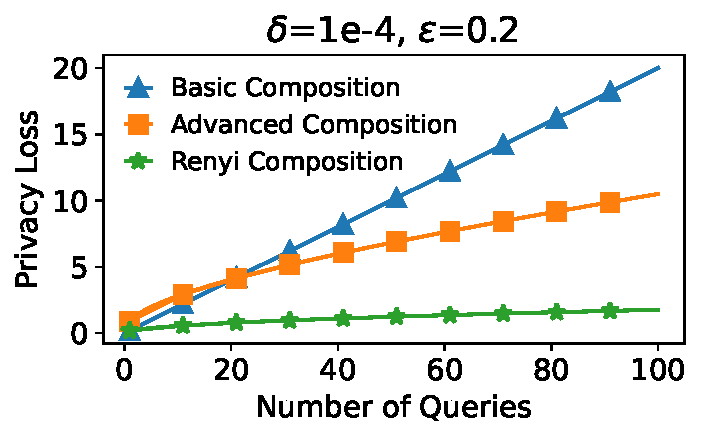
\includegraphics[width=\columnwidth]{plots/composition_comparison.pdf}
  \caption{Aggregated privacy loss of multiple queries reported by different composition methods}
  \label{fig:composition-comparison}
\end{figure}

\Cref{fig:composition-comparison} compares different methods for composing privacy loss of DP mechanisms.
We can see the effectiveness of R\'enyi methods compared to others across all the values for number of queries.
The advanced composition theorem also outperforms the basic composition theorem at large number of queries. 


As we mentioned earlier, $(\alpha, \varepsilon)$-RDP is strictly stronger than $\varepsilon, \delta$-DP. 
The next proposition shows how RDP implies standard DP.
\begin{proposition}\label{prop:rdp-better-than-dp}
  If $M: \dbSpace \rightarrow \mathbb{R}$ is an $(\alpha, \varepsilon)$-RDP mechanism, it is also $(\varepsilon + \frac{\log 1/\delta}{\alpha-1}, \delta)$-DP for any $0 < \delta < 1$. 
\end{proposition}
\noindent \Cref{prop:rdp-better-than-dp} enables us to interpret guarantees of R\'enyi differential privacy with the semantics of standard differential privacy. 
Besides that, \Cref{prop:rdp-composition} provides us with the means to compose heterogeneous differentially private algorithms, while with \Cref{prop:rdp-better-than-dp} we can still represent the final result using the semantics of standard DP. 
To compute the privacy loss (\ie $\varepsilon$) of our differentially private shaping mechanism in \Cref{sec:dp-privacy-guarantees}, we use \Cref{prop:rdp-composition} referred to as $\textrm{DP\_compose}()$.